\documentclass[titlepage=firstiscover, bibliography=totoc, captions=tableheading]{scrartcl}
\author{Felix Geyer \\
  \texorpdfstring{\href{mailto:felix.geyer@tu-dortmund.de}{felix.geyer@tu-dortmund.de}\and}{,}
  Rune Dominik \\
  \texorpdfstring{\href{mailto:rune.dominik@tu-dortmund.de}{rune.dominik@tu-dortmund.de}}{}
  }
\title{V354: Gedämpfte und erzwungene Schwingungen}
\date{Durchführung: 10. Januar 2017 \\
      Abgabe: 17. Januar 2017}
\usepackage[aux]{rerunfilecheck}
\usepackage{polyglossia}
\setmainlanguage{german}
\usepackage{amsmath}
\usepackage{amssymb}
\usepackage{mathtools}
\usepackage{fontspec}

\usepackage{scrhack}
\usepackage{float}
\floatplacement{table}{htbp}
\floatplacement{figure}{htbp}

\usepackage[locale=DE, separate-uncertainty=true, per-mode=symbol-or-fraction, decimalsymbol=.]{siunitx}
%\usepackage{siunitx}

\usepackage[style=alphabetic]{biblatex}
\addbibresource{lit.bib}

\usepackage[section, below]{placeins}
\usepackage[labelfont=bf,
font=small,
width=0.9\textwidth,
format=plain,
indention=1em]{caption}
\usepackage{graphicx}
\usepackage{grffile}
\usepackage{subcaption}

\usepackage[math-style=ISO, bold-style=ISO, sans-style=italic, nabla=upright, partial=upright]{unicode-math}
\setmathfont{Latin Modern Math}

\usepackage[autostyle]{csquotes}

\usepackage[unicode]{hyperref}

\usepackage{bookmark}

\usepackage{booktabs}

\begin{document}
\begin{titlepage}
  \begin{flushleft}
 Durchführung: 15.05.2018\\
 Abgabe: 22.05.2018
  \end{flushleft}


%\HRule\\[1,0cm]

 \begin{center}


\textsc{\LARGE Praktikumsprotokoll V606}\\[1.5cm]
\textsc{\huge Suszeptibilität paramagnetischer Substanzen} \\[5,5cm]

Carolin Harkort\footnotemark[1], \\
Jacqueline Schlingmann\footnotemark[2] \\[1,0cm]



 \end{center}
%\HRule

 \vfill

 \footnotetext[1]{\href{mailto:carolin.harkort@tu-dortmund.de}{carolin.harkort@tu-dortmund.de}}
 \footnotetext[2]{\href{mailto:jacqueline.schlingmann@tu-dortmund.de}{jacqueline.schlingmann@tu-dortmund.de}}
\end{titlepage}


  
\section{Zielsetzung}
Ziel des Versuchs ist die Bestimmung unbekannter Brennweiten.

\section{Theorie}
Trifft Licht auf eine Linse wird dieses gebrochen.
Man unterscheidet zwischen Sammel- und Zerstreuungslinsen.
Sammellinsen bündeln paralleles Licht und es entsteht ein reelles Bild.
Die Brennweite und die Bildweite sind hierbei positiv.
Eine Sammellinse ist in Abbildung (\ref{fig:sam}) zu sehen.

\begin{figure}
\centering
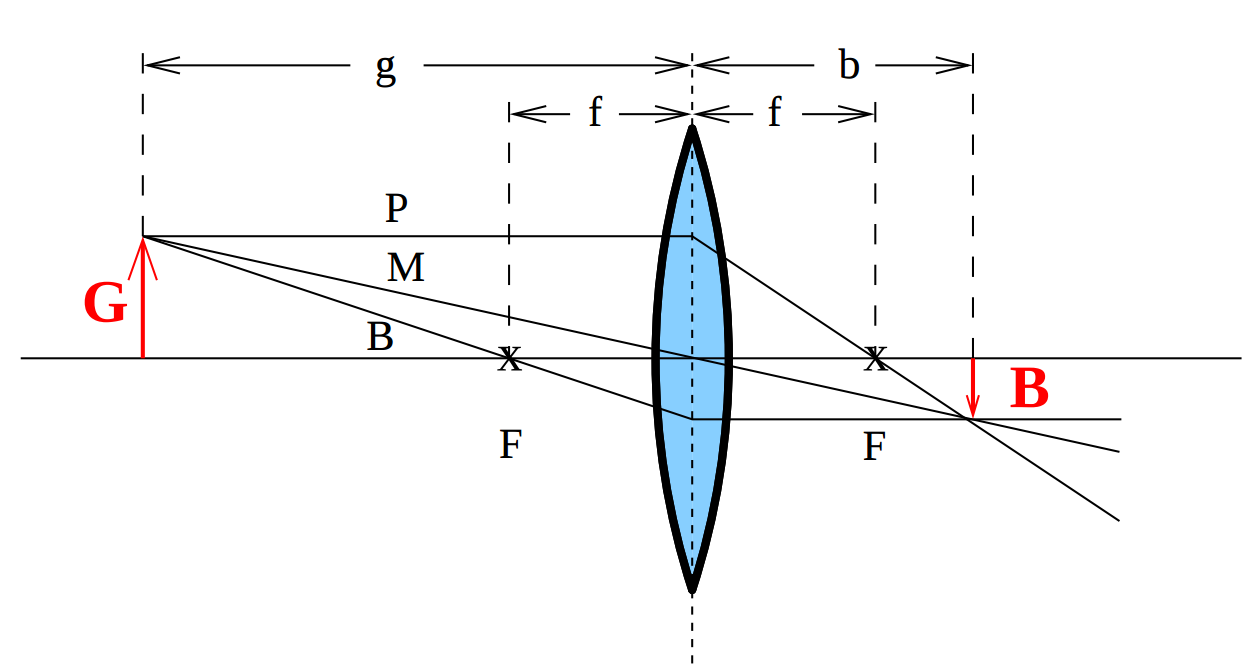
\includegraphics[height=4.60cm]{sammellinse.png}
\caption{Die Sammellinse}\cite{on1}
\label{fig:sam}
\end{figure}

Bei der Zerstreuungslinse sind Brenn- und Bildweite negativ,
sodass ein virtuelles Bild entsteht.
Sie ist in abbildung (\ref{fig:zer}) zu sehen.


\begin{figure}
\centering
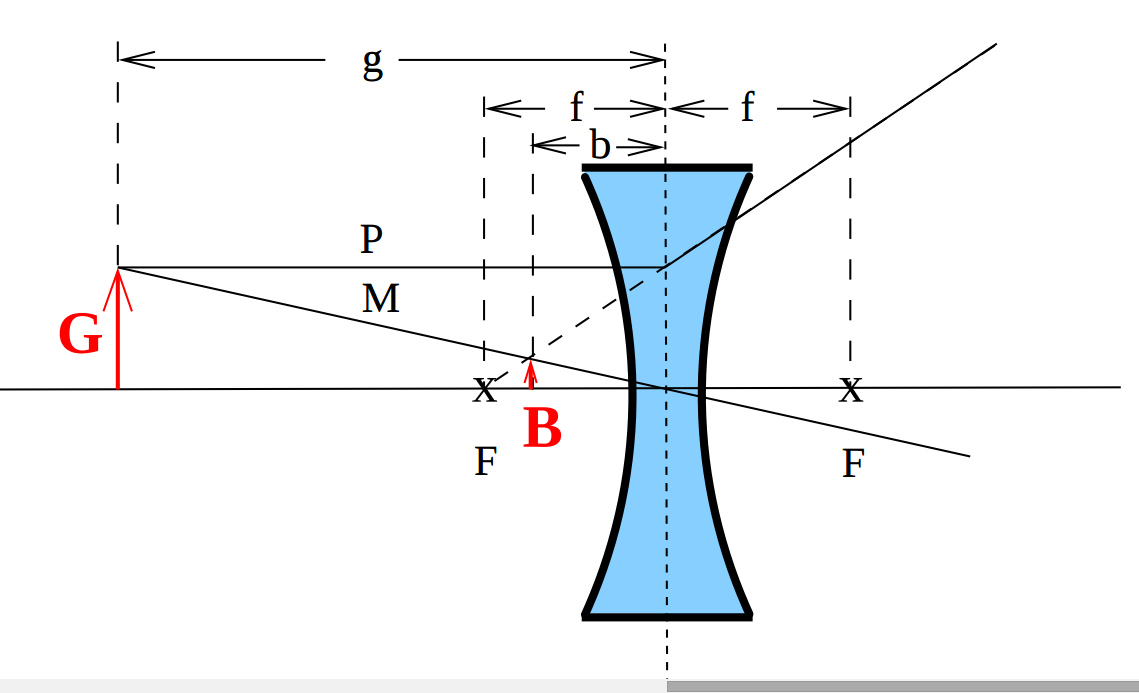
\includegraphics[height=4.60cm]{zerstreungslinse.png}
\caption{Die Zerstreuungslinse}\cite{on1}
\label{fig:zer}
\end{figure}

Für die Bildkonstruktion werden drei unterschiedliche Strahlen verwendet.\\
\emph{Parallelstrahl (P)}: Dieser verläuft Parallel zur optischen Achse und wird dann an
der Mittelebene so gebrochen, dass er durch den Brennpunkt verläuft.\\
\emph{Brennpunktstrahl (B)}: Dieser verläuft umgekehrt zum Parallelstrahl.
Er verläuft zunächst durch den Brennpunkt zur Mittelebene der Linse
und wird dann so gebrochen, dass er parallel zur optischen Achse verläuft.\\
\emph{Mittelpunktstrahl (M)}: Dieser Strahl verläuft direkt durch die Mitte,
also durch den Schnittpunkt zwischen der optischen Achse und der Mittelpunktebene.
Er wird nicht gebrochen.

Das Abbildungsgesezt
\begin{equation}
  V = \frac{B}{G}=\frac{b}{g}
  \label{eqn:abbgesetz}
\end{equation}
ergibt sich aus den Strahlensätzen und der Bildkonstruktion.
Hierbei ist V der Abbildungsmaßstab, B und G die Bild- bzw. Gegenstandsgröße und
b und g die Bild- bzw. Gegenstandsweite.
Aus dem Abbildungsgesetz folgt auch die Linsengeichung:
\begin{equation}
  \frac{1}{f}= \frac{1}{b}+\frac{1}{g}
  \label{eqn:linsgl}
\end{equation}
\subsubsection{Bestimmung der Brennweite nach der Methode von Bessel}
Bei der Methode von Bessel werden die Beiden Linsenpositionen gesucht,
an denen das Bild scharf abgebildet wird.
Dies geschieht bei konstantem Abstand zwischen Bild und Gegenstand.
Die Brennweite ergibt sich mit der Formel
\begin{equation}
  f = \frac{e^2 - d^2}{4e} .
  \label{eqn:fe}
\end{equation}
Hierbei ist e der Abstand zwischen Bild und Gegenstand und d der Abstand zwischen den beiden Lisenositionen.
Für d gilt:
\begin{equation}
  d= g_1-b_1 = g_2-b_2
  \label{eqn:d}
\end{equation}
\subsubsection{Bestimmung der Brennweite nach Abbe }
Bei der Brennweitenbestimmung nach Abbe sind zwei Linsen hintereinander angebracht.
Darum muss eine Hauptebene eingeführt werden, an der der Strah gebrochen wird.
Dies h und die Brennweite f bestimmt sich durch Formel
\begin{equation*}
  g' = g+h = f \cdot \left(1 + \frac{1}{V}\right)+h
\end{equation*}
bzw.
\begin{equation}
  b' = b+h'= f\cdot(1+V) +h'
\end{equation}
\section{Durchführung}

Die Apparatur besteht aus einer Lichtquelle und einer Schiene.
Auf der Schiene ist ein Schirm befestigt, auf dem das Bild abgebildet wird,
und eine Befestigungsvorrichtung zum Einsetzen der Linsen. Der Gegenstand,
der abgebildet werden soll, ist ebenfall auf der Schiene befestigt.
Er besteht aus einer schwarzen Scheibe mit lichtdurchlässigen Löchern, die ein 'L' ergeben.

Im ersten Teil des Veruchs wurde eine Sammellinse in der Apparatur befestigt.
Der Abstand zwischen Lichtquelle und Gegenstand wird notiert und konstant gehalten.
Die Sammellinse wird nun auf zehn unterschiedliche Entfernungen zum Gegenstand gebracht.
Zu jedem Abstand wird geguckt,
bei welcher Entfernung des Schirms zur Sammellinse das Bild scharf dargestellt wird.
Diese Messung wird für zwei unterschiedliche Sammellinsen durchgeführt.

Im zweiten Teil des Versuchs wird ebenfalls eine Sammellinse benötigt.
Die Bestimmung der Brennweite erfolgt nach der Methode von Bessel.
Der abzubildende Gegenstand wird wieder auf einem konstanten Abstand zur Lichtquelle gehalten.
Das Bild bei dieser Messung ebenfalls.
Es werden die beiden Linsenpositionen gesucht, bei der ein scharfes Bild entsteht.
Danach wird eine rot bzw. blaue Scheibe am Gegenstand befestigt.
Die Messung wird für beide Farben fünf mal wiederholt.

Im letzten Teil des Versuchs wurde nun eine Zerstreuunglinse vor der Sammellinse befestigt.
Dies ist in Abbildung (\ref{fig:linsys}) zu sehen.
Die Messung erfolgt nach der Methode von Abbe
Die Durchführung ähnelt der des ersten Teils.
\begin{figure}
\centering
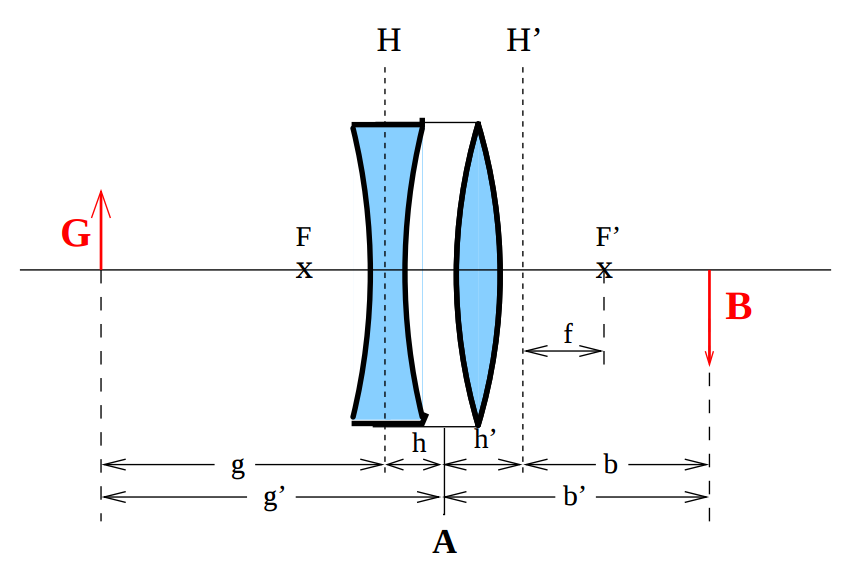
\includegraphics[height=4.60cm]{linsensystem.png}
\caption{Das Linsensystem}\cite{on1}
\label{fig:linsys}
\end{figure}

  %\input{durchführung.tex}
  \section{Auswertung}
Zu Anfang wird die Leerlaufsannung einer Monozelle bestimmt
und der Innenwiderstand vom Amperemeter abgelesen.
\begin{align*}
  U &= 1,47\, \mathrm{V} & R_I &= 10\, \mathrm{M\Omega}
\end{align*}
Im folgenden werden für die drei Spannungsquellen die Spannung $U_0$ und
der Widerstand $R_i$ bestimmt.
Dafür werden die gemessenen Werte für die Klemmspannung $U_k$
gegen die Werte für den Strom $I$ aufgetragen.
Diese Werte sind in den Tabellen (\ref{tab:1}), (\ref{tab:2}), (\ref{tab:3})
und (\ref{tab:4}) zu finden.
Der Wert für die Steigung der folgenden linearen Ausgleichsgraden,
beschreibt den Wert des Innenwiderstandes. Die Verschiebung auf der y-Achse
beschreibt den Wert für $U_0$
\subsection{Monozelle ohne Gegenspannung}
Die Werte für $R_i$ und $U_0$ für eine Monozelle ohne Gegenspannung,
werden wie oben beschrieben ermittelt und lauten:
\begin{align}
  R_i &= (15,60 \pm 0,16)\, \mathrm{\Omega}\\
  \label{eqn:ri}
  U_0 &= (1,519 \pm 0,008)\, \mathrm{V}
\end{align}
Die Regression ist in Abbidung (\ref{fig:Messunga}) zu sehen.
\begin{table}
  \centering
  \caption{Messwerte für eine Monozelle ohne Gegenspannung}
  \label{tab:1}
  \begin{tabular}{c c }
    \toprule $I/A$ & $U/V$ \\
    \midrule
    0,092 & 0,09\\
    0,070 & 0,42\\
    0,059 & 0,60\\
    0,0495 & 0,75\\
    0,043 & 0,84\\
    0,037 & 0,93\\
    0,033 & 1,02\\
    0,029 & 1,05\\
    0,027 & 1,11\\
    0,024 & 1,14\\
    0,023 & 1,17\\
    \bottomrule
  \end{tabular}
\end{table}

\begin{figure}[H]
  \centering
  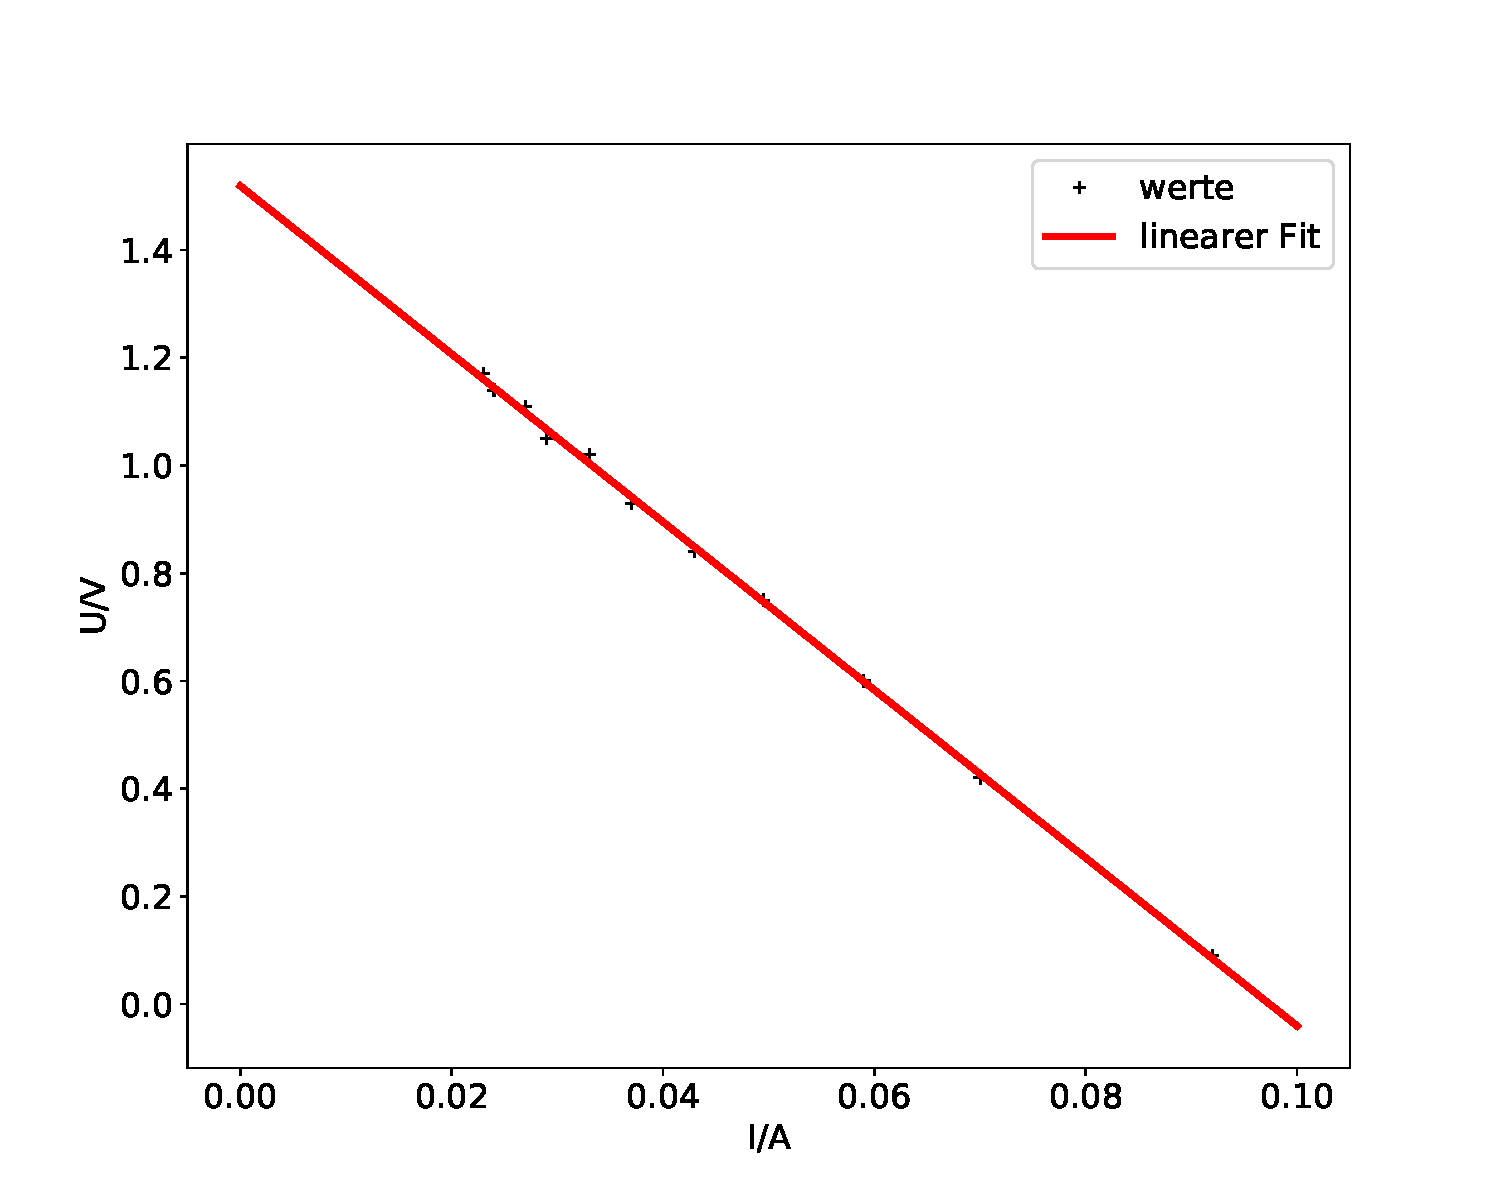
\includegraphics[width=\textwidth]{plota.pdf}
  \caption{Monozelle ohne Gegenspannung}
  \label{fig:Messunga}
\end{figure}
\subsection{Monozelle mit Gegenspannung}
Ist an der Monozelle eine Gegenspannung angelegt,
ergeben sich folgende Werte für $R_i$ und $U_0$:
\begin{align*}
  R_i &= (4,80 \pm 0,22)\, \mathrm{\Omega}\\
  U_0 &= (0,467 \pm 0,013)\, \mathrm{V}
\end{align*}
Die lineare Regression ist in Abbildung (\ref{fig:Messungb}) gezeigt.
\begin{table}
  \centering
  \caption{Messwerte für eine Monozelle mit Gegenspannung}
  \label{tab:2}
  \begin{tabular}{c c}
    \toprule $I/mA$ & $U/V$ \\
    \midrule
    99 & 0,96\\
    91 & 0,87\\
    68 & 0,81\\
    58 & 0,75\\
    51 & 0,72\\
    46 & 0,69\\
    41 & 0,66\\
    37 & 0,64\\
    34 & 0,63\\
    33 & 0,62\\
    \bottomrule
  \end{tabular}
\end{table}

\begin{figure}[H]
  \centering
  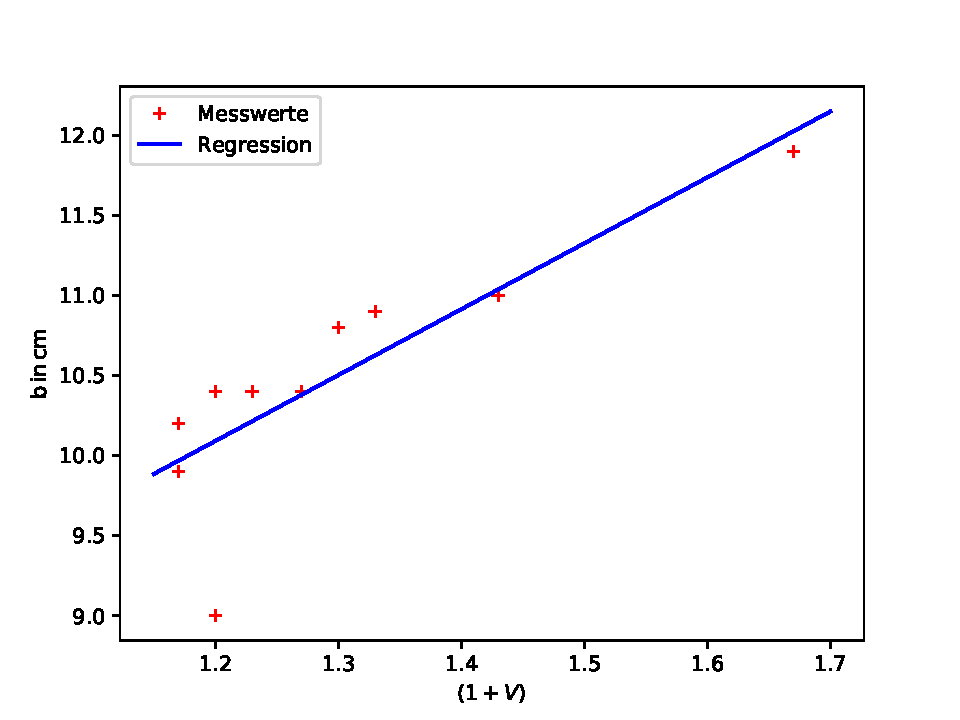
\includegraphics[width=\textwidth]{plotb.pdf}
  \caption{Monozelle mit Gegenspannung}
  \label{fig:Messungb}
\end{figure}

\subsection{Rechteck- und Sinusspannung}
Für die Rechteck- und Sinusspannung wird die Regression
und die Bestimmung von $U_0$ und $R_i$ ebenfalls wie oben bestimmt.
\begin{table}
  \centering
  \caption{gemessene Werte zur Rechteckspannung}
  \label{tab:3}
  \begin{tabular}{c c}
    \toprule $I/mA$ & $U/V$  \\
    \midrule
    8,0 & 0,19\\
    7,1 & 0,23\\
    5,7 & 0,32\\
    4,4 & 0,38\\
    3,6 & 0,42\\
    3,2 & 0,45\\
    2,8 & 0,47\\
    2,5 & 0,49\\
    2,2 & 0,50\\
    2,0 & 0,52\\
    1,8 & 0,53\\
    \bottomrule
  \end{tabular}
\end{table}
Für die Rechteckspannung lauten die Werte:
\begin{align*}
  R_i &= (54,8 \pm 0,8)\, \mathrm{\Omega}\\
  U_0 &= (0,6249 \pm 0,0034)\, \mathrm{V}
\end{align*}
Die Regression ist in Abbildung (\ref{fig:c}) zu sehen.

\begin{figure}[H]
  \centering
  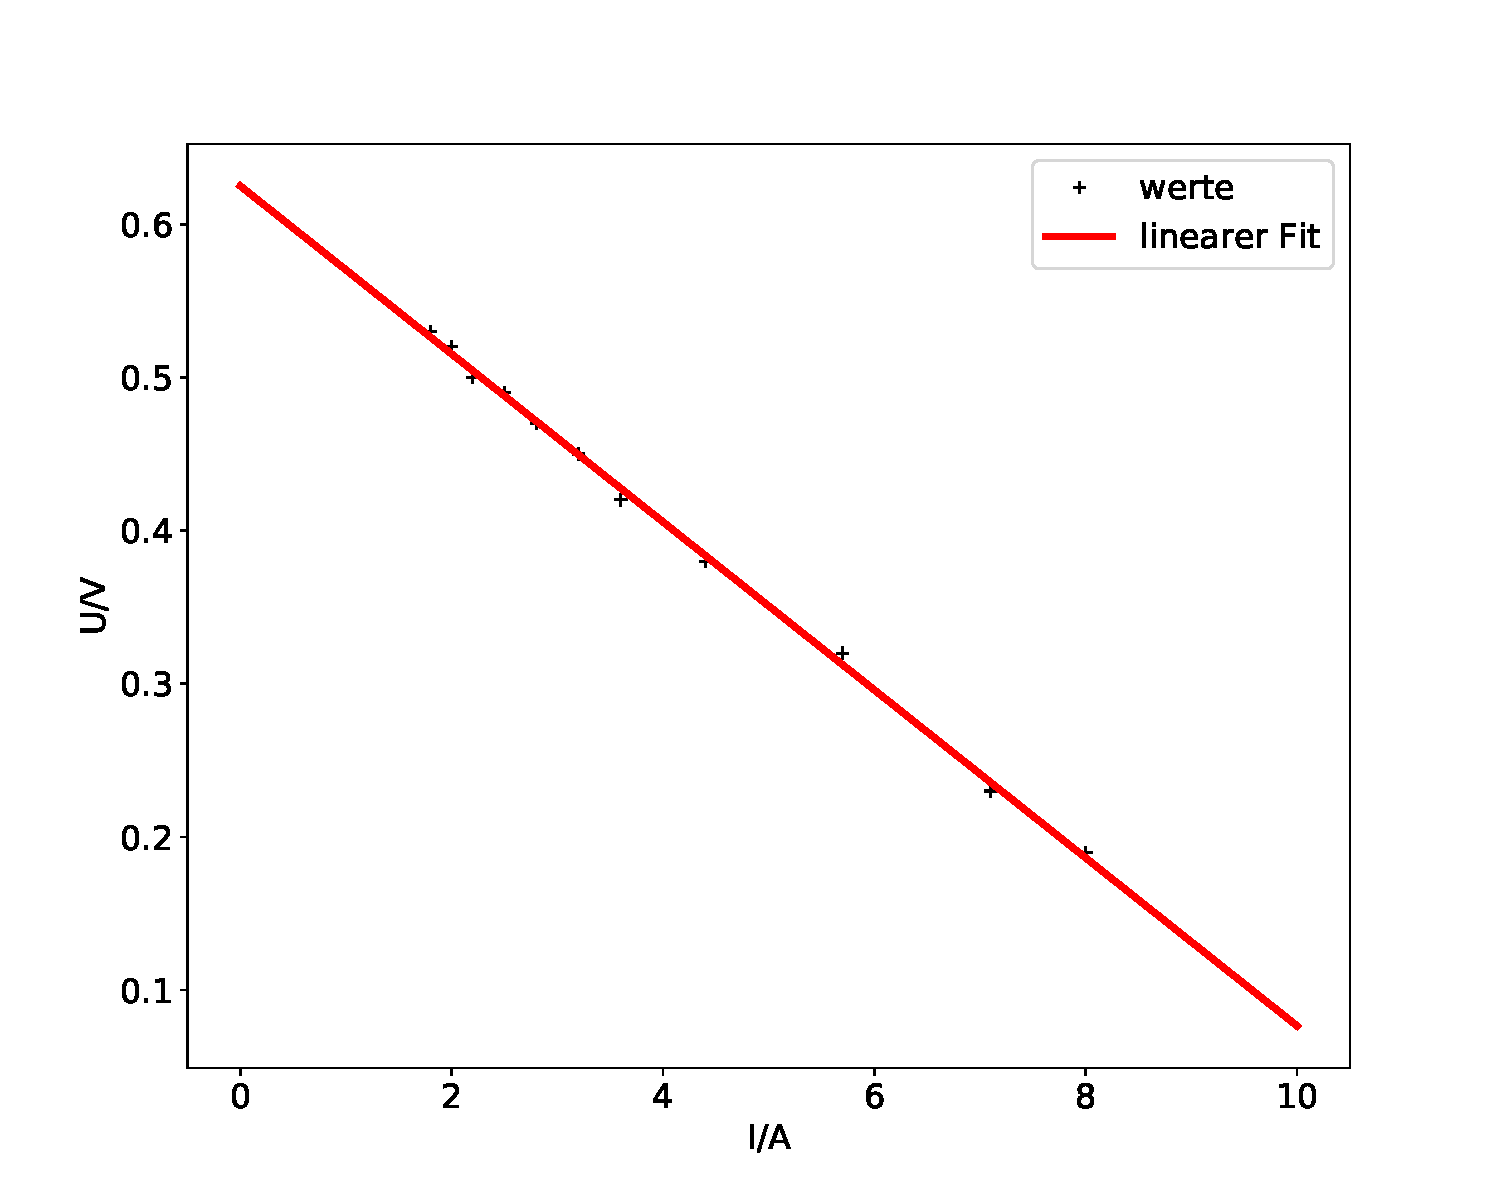
\includegraphics[width=\textwidth]{plotreck.pdf}
  \caption{Monozelle ohne Gegenspannung}
  \label{fig:c}
\end{figure}

\begin{table}
  \centering
  \caption{gemessene Werte zur Sinusspannung}
  \label{tab:4}
  \begin{tabular}{c c}
    \toprule $I/mA$ & $U/V$  \\
    \midrule
    0,97 & 0,41\\
    0,66 & 0,62\\
    0,50 & 0,73\\
    0,39 & 0,81\\
    0,34 & 0,85\\
    0,28 & 0,88\\
    0,24 & 0,91\\
    0,20 & 0,94\\
    0,18 & 0,96\\
    0,16 & 0,97\\
    \bottomrule
  \end{tabular}
\end{table}
Die Werte für die Sinusspannung lauten:
\begin{align*}
  R_i &= (693 \pm 5)\, \mathrm{\Omega}\\
  U_0 &= (1,0795 \pm 0,0024)\, \mathrm{V}
\end{align*}
die lineare Regression ist in Abbildung (\ref{fig:d}) gezeigt.
  \begin{figure}[H]
    \centering
    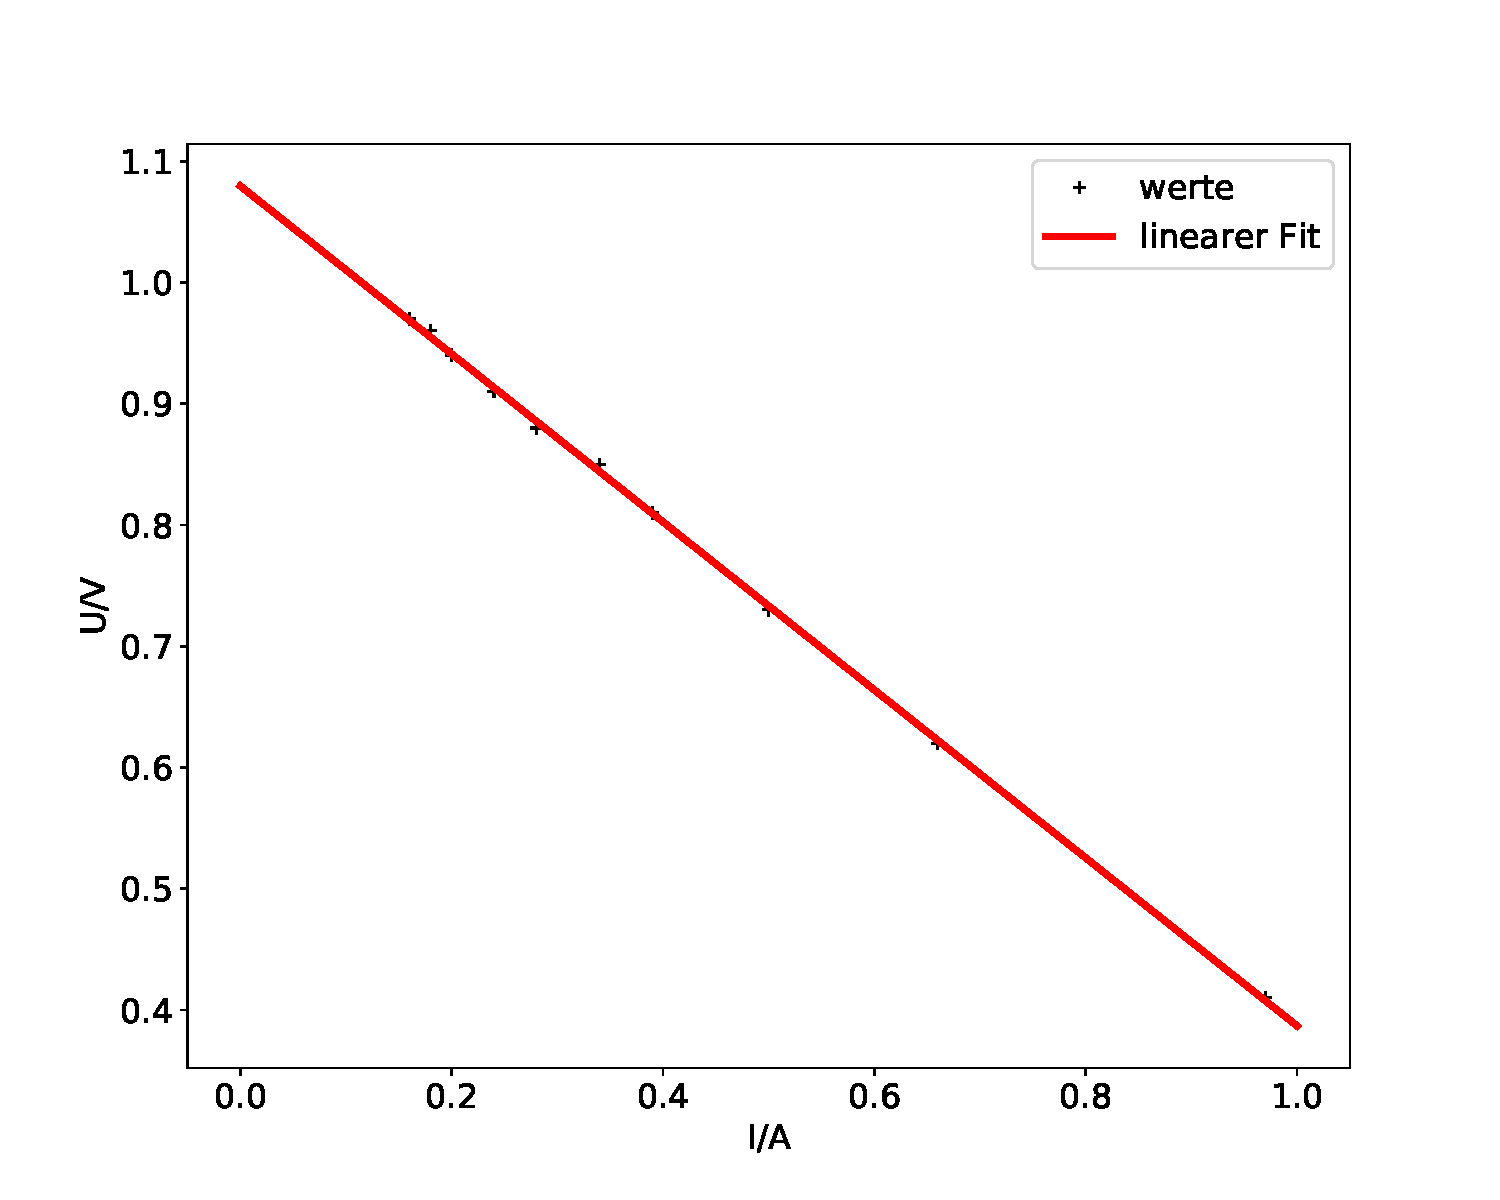
\includegraphics[width=\textwidth]{plotsin.pdf}
    \caption{Monozelle ohne Gegenspannung}
    \label{fig:d}
  \end{figure}
Die verwendeten Messwerte sind in den Tabellen (\ref{tab:3}) und (\ref{tab:4}) zu finden.

  \subsection{Systematischer Fehler der $U_0$ Messung}

Der systematische Fehler der $U_0$-Messung entsteht aufgrund des Eigenwiderstandes
des verwendeten Voltmeters.
Dieser wird vom Gerät abgelesen und liegt bei $10\, M\Omega$
Der Fehler wird mit der Formel
\begin{equation}
  \Delta U = U_K \cdot \frac{R_i}{R_v}\,\, := f
\end{equation}
berechnet. $U_K$ ist die Klemmspannung und wurde zu Anfang abgelesen.
Sie liegt bei $1,47 \, V$. \\
$R_i$ entspricht den in \ref{eqn:ri} berechneten Innenwiderstand.
\\
Der fehler ergibt sich durch Formel:
\begin{equation*}
  \Delta f = \frac{U_K}{R_v}\cdot\Delta R_i
\end{equation*}
Somit berechnet sich der Fehler zu
\begin{equation*}
  \Delta U = (2,2932 \pm 0,0235) \cdot 10^{-6} \mathrm{V}\, .
\end{equation*}

\subsection{Im Belastungswiderstand umgesetzte Leistung der Monozelle}
Die im Belastungswiderstand umgesetzte Leistung wird ermittelt,
indem $U \cdot I$ gegen $U/I$ aufgetragen wird.
Die Werte sind in Tabelle (\ref{tab:lei}) zu finden.
\begin{table}
  \centering
  \caption{n}
  \label{tab:lei}
  \begin{tabular}{c c c c}
    \toprule $I/A$ & $U/V$ & $(U\cdot I)/W$ & $(U/I)/\Omega$\\
    \midrule
    0,092 & 0,09 & 0,0083 & 0,978\\
    0,070 & 0,42 & 0,0294 & 6,00\\
    0,059 & 0,60 & 0,0354 & 10,17\\
    0,0495 & 0,75 & 0,0371 & 15,15\\
    0,043 & 0,84 & 0,0361 & 19,53\\
    0,037 & 0,93 & 0,0344 & 25,14\\
    0,033 & 1,02 & 0,0337 & 30,90\\
    0,029 & 1,05 & 0,0305 & 36,21\\
    0,027 & 1,11 & 0,0299 & 41,11\\
    0,024 & 1,14 & 0,0274 & 47,50\\
    0,023 & 1,17 & 0,0269 & 50,87\\
    \bottomrule
  \end{tabular}
\end{table}
In Abbildung (\ref{fig:fite}) sind die Werte aufgetragen.
Außerdem wurde eine Theoriekurve mit der Formel
\begin{equation*}
  N(R_a)= \frac{ U_0^2 \cdot R_a}{(R_i + R_a)^2}
\end{equation*}
eingefügt, um systematische Fehler zu ermitteln.
\begin{figure}[H]
  \centering
  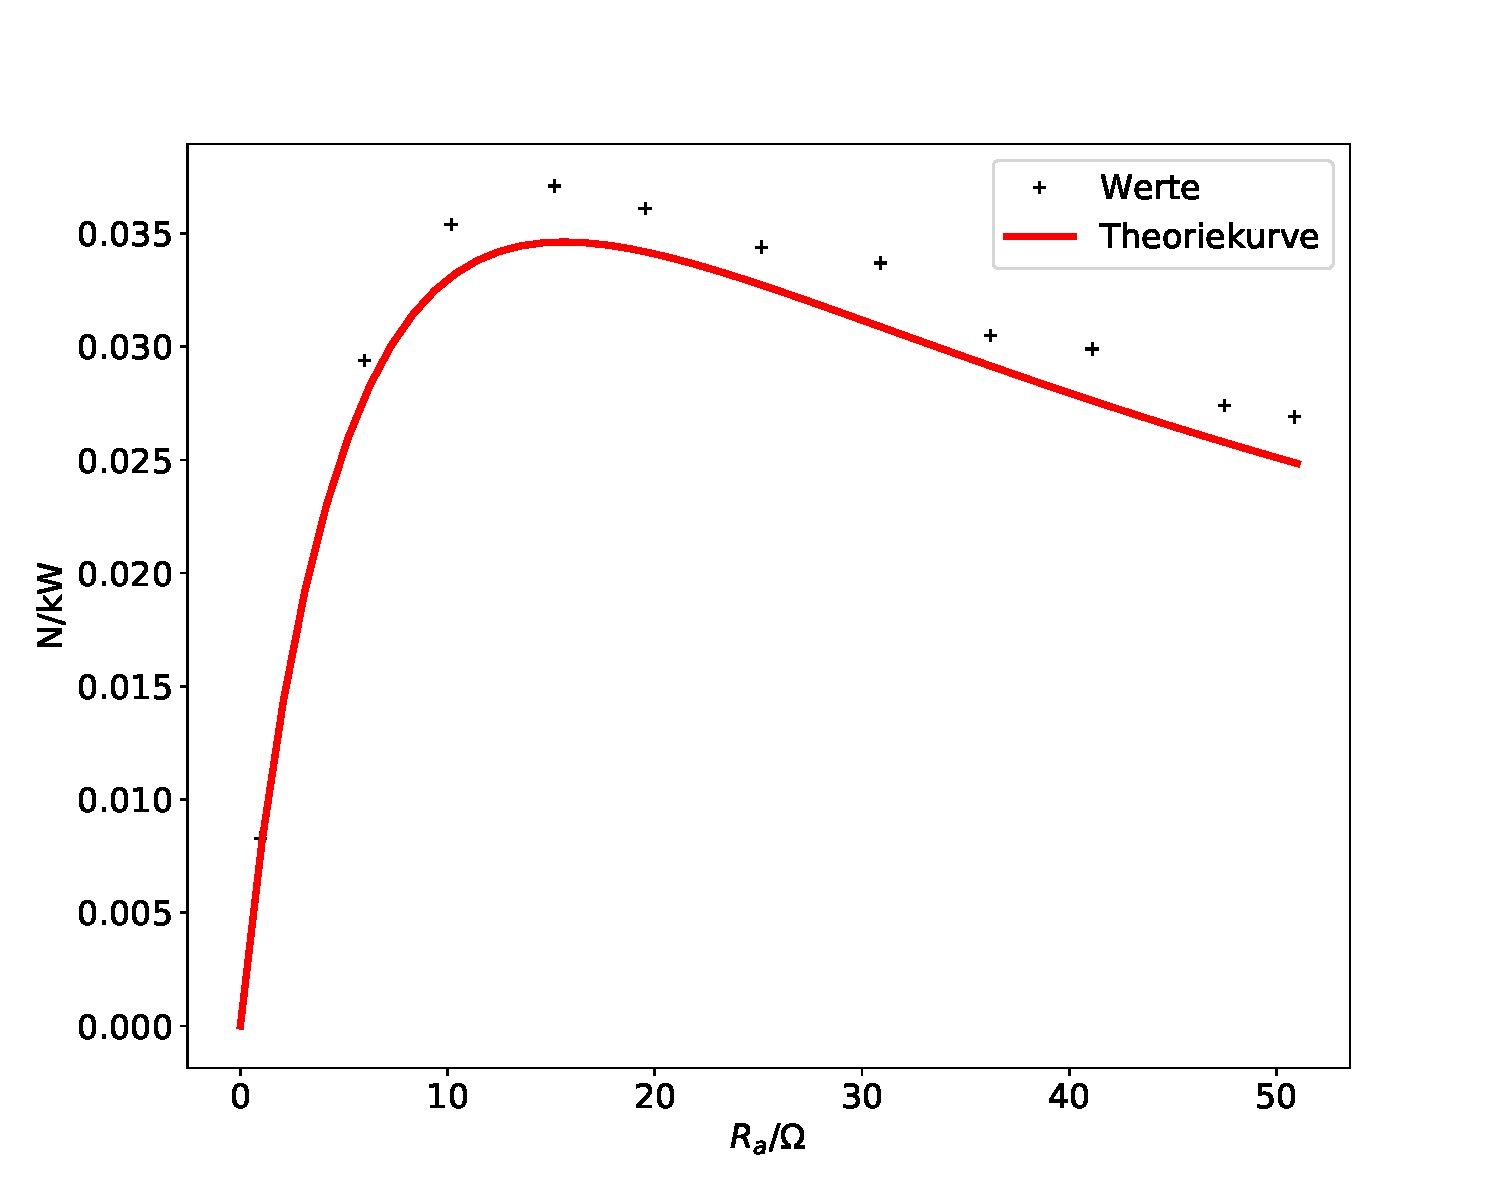
\includegraphics[width=\textwidth]{plote.pdf}
  \caption{Leistungsabfall am Belastungswiderstand}
  \label{fig:fite}
\end{figure}
Die meisten Messwerte liegen über der Kurve.
Allerdings liegt die abweichung bei ca. $0,002\, V$, sodass nicht davon auszugehen ist,
dass  ein systematischer Fehler gemacht wurde.
Das Maximum der Kurve liegt vor, wenn $R_a = R_i$
und stimmt sehr gut mit den gemessenen Werten überein.

\section{Diskussion}

In den Abbildungen der linearen Regressionen ist gut zu erkennen,
dass die Messwerte gegenüber der Ausgleichsgrade nur leicht Abweichen
und im Bereich der Messungenauigkeiten liegen.
somit ist davon auszugehen, dass keine größeren Systematischen Fehler begangen wurden.
Es fällt allerdings auf, dass die gemessene Spannung $U_0$ und der Widerstand $R_i$ einer Monozelle
 mit Gegenspannung sehr klein sind.
 Dieses Ergebnis wurde nicht erwartet und könnte an einem Fehler im Aufbau der Schaltung liegen.
 Das Amperemeter sollte hinter das Voltmeter geschaltet werden.
 Wird dieses andersherum aufgebaut, wirkt der Eigenwiderstand des Amperemeter
 und verringert den Wert der Messung sehr stark.


\nocite{*}
\printbibliography
\end{document}
